%% BioMed_Central_Tex_Template_v1.06
%%                                      %
%  bmc_article.tex            ver: 1.06 %
%                                       %

%%IMPORTANT: do not delete the first line of this template
%%It must be present to enable the BMC Submission system to
%%recognise this template!!

%%%%%%%%%%%%%%%%%%%%%%%%%%%%%%%%%%%%%%%%%
%%                                     %%
%%  LaTeX template for BioMed Central  %%
%%     journal article submissions     %%
%%                                     %%
%%          <8 June 2012>              %%
%%                                     %%
%%                                     %%
%%%%%%%%%%%%%%%%%%%%%%%%%%%%%%%%%%%%%%%%%


%%%%%%%%%%%%%%%%%%%%%%%%%%%%%%%%%%%%%%%%%%%%%%%%%%%%%%%%%%%%%%%%%%%%%
%%                                                                 %%
%% For instructions on how to fill out this Tex template           %%
%% document please refer to Readme.html and the instructions for   %%
%% authors page on the biomed central website                      %%
%% http://www.biomedcentral.com/info/authors/                      %%
%%                                                                 %%
%% Please do not use \input{...} to include other tex files.       %%
%% Submit your LaTeX manuscript as one .tex document.              %%
%%                                                                 %%
%% All additional figures and files should be attached             %%
%% separately and not embedded in the \TeX\ document itself.       %%
%%                                                                 %%
%% BioMed Central currently use the MikTex distribution of         %%
%% TeX for Windows) of TeX and LaTeX.  This is available from      %%
%% http://www.miktex.org                                           %%
%%                                                                 %%
%%%%%%%%%%%%%%%%%%%%%%%%%%%%%%%%%%%%%%%%%%%%%%%%%%%%%%%%%%%%%%%%%%%%%

%%% additional documentclass options:
%  [doublespacing]
%  [linenumbers]   - put the line numbers on margins

%%% loading packages, author definitions

%\documentclass[twocolumn]{bmcart}% uncomment this for twocolumn layout and comment line below
\documentclass{bmcart}

%%% Load packages
\usepackage{amsthm,amsmath}
\RequirePackage{natbib}
%\RequirePackage[authoryear]{natbib}% uncomment this for author-year bibliography
\RequirePackage{hyperref}
\usepackage[utf8]{inputenc} %unicode support
%\usepackage[applemac]{inputenc} %applemac support if unicode package fails
%\usepackage[latin1]{inputenc} %UNIX support if unicode package fails
%\usepackage{siunitx}
\usepackage[colorlinks]{hyperref} % To color blocks of text 
%\usepackage[dvipsnames]{xcolor} % More color options (see Wikibooks)  
\usepackage{changepage}
\usepackage{booktabs} % For prettier tables
\usepackage{float} % To control positions of e.g. tables or figures
%\usepackage[section]{placeins}
\usepackage{graphicx}
\usepackage[flushleft]{threeparttable}

% to color table rows
\usepackage{color, colortbl}
\graphicspath{ {../} }

%%%%%%%%%%%%%%%%%%%%%%%%%%%%%%%%%%%%%%%%%%%%%%%%%
%%                                             %%
%%  If you wish to display your graphics for   %%
%%  your own use using includegraphic or       %%
%%  includegraphics, then comment out the      %%
%%  following two lines of code.               %%
%%  NB: These line *must* be included when     %%
%%  submitting to BMC.                         %%
%%  All figure files must be submitted as      %%
%%  separate graphics through the BMC          %%
%%  submission process, not included in the    %%
%%  submitted article.                         %%
%%                                             %%
%%%%%%%%%%%%%%%%%%%%%%%%%%%%%%%%%%%%%%%%%%%%%%%%%

%\def\includegraphic{}
%\def\includegraphics{}



%%% Put your definitions there:
\startlocaldefs
\endlocaldefs


%%% Begin ...
\begin{document}

%%% Start of article front matter
\begin{frontmatter}

\begin{fmbox}
\dochead{Research}

%%%%%%%%%%%%%%%%%%%%%%%%%%%%%%%%%%%%%%%%%%%%%%
%%                                          %%
%% Enter the title of your article here     %%
%%                                          %%
%%%%%%%%%%%%%%%%%%%%%%%%%%%%%%%%%%%%%%%%%%%%%%

\title{Dual host-parasite transcriptomes of apicomplexan Eimeria
  falciformis and its natural mouse host}

%%%%%%%%%%%%%%%%%%%%%%%%%%%%%%%%%%%%%%%%%%%%%%
%%                                          %%
%% Enter the authors here                   %%
%%                                          %%
%% Specify information, if available,       %%
%% in the form:                             %%
%%   <key>={<id1>,<id2>}                    %%
%%   <key>=                                 %%
%% Comment or delete the keys which are     %%
%% not used. Repeat \author command as much %%
%% as required.                             %%
%%                                          %%
%%%%%%%%%%%%%%%%%%%%%%%%%%%%%%%%%%%%%%%%%%%%%%
%%%%%%%%%%%%%%%%%%%%%%%%%%%%

\author[ addressref={aff1},] {\inits{TK}\fnm{Totta} \snm{Kasemo}}
\author[ addressref={aff1},] {\inits{SS}\fnm{Simone} \snm{Spork}}
\author[ addressref={aff2},] {\inits{CD}\fnm{Christoph} \snm{Dieterich}}
\author[ addressref={aff1}, ]{\inits{RL}\fnm{Richard} \snm{Lucius}}
\author[ addressref={aff1, aff3},              
  corref={aff1},                   
  email={emanuel.heitlinger@hu-berlin.de}]{\inits{EH}\fnm{Emanuel} \snm{Heitlinger}}

%%%%%%%%%%%%%%%%%%%%%%%%%%%%%%%%%%%%%%%%%%%%%%
%%                                          %%
%% Enter the authors' addresses here        %%
%%                                          %%
%% Repeat \address commands as much as      %%
%% required.                                %%
%%                                          %%
%%%%%%%%%%%%%%%%%%%%%%%%%%%%%%%%%%%%%%%%%%%%%%

\address[id=aff1]{
	\orgname{Institute of Biology, Humboldt-Universitat zu Berlin}, 
	\street{Philippstr. 13, Haus 14},
	\postcode{10115}                 
	\city{Berlin},                   
	\cny{Germany}                    
}
\address[id=aff2]{  
	\orgname{Max Planck Institute for Biology of Ageing},
	\street{Joseph-Stelzmann-Strasse 9B},
	\postcode{50931}
	\city{Cologne},
	\cny{Germany}
}
\address[id=aff3]{  
	\orgname{Leibniz Institute of Zoo and Wildlife Research},
	\street{Alfred-Kowalke-Str. 17},
	\postcode{10315}
	\city{Berlin},
	\cny{Germany}
}

%%%%%%%%%%%%%%%%%%%%%%%%%%%%%%%%%%%%%%%%%%%%%%
%%                                          %%
%% Enter short notes here                   %%
%%                                          %%
%% Short notes will be after addresses      %%
%% on first page.                           %%
%%                                          %%
%%%%%%%%%%%%%%%%%%%%%%%%%%%%%%%%%%%%%%%%%%%%%%

\begin{artnotes}
%\note{Sample of title note}     % note to the article
%\note[id=n1]{Equal contributor} % note, connected to author
%\note[id=n2]
\end{artnotes}

%\end{fmbox}% comment this for two column layout

%%%%%%%%%%%%%%%%%%%%%%%%%%%%%%%%%%%%%%%%%%%%%%
%%                                          %%
%% The Abstract begins here                 %%
%%                                          %%
%% Please refer to the Instructions for     %%
%% authors on http://www.biomedcentral.com  %%
%% and include the section headings         %%
%% accordingly for your article type.       %%
%%                                          %%
%%%%%%%%%%%%%%%%%%%%%%%%%%%%%%%%%%%%%%%%%%%%%%

\begin{abstractbox}

\begin{abstract} % abstract
\parttitle{First part title} %if any
Text for this section.

\parttitle{Second part title} %if any
Text for this section.
\end{abstract}

%%%%%%%%%%%%%%%%%%%%%%%%%%%%%%%%%%%%%%%%%%%%%%
%%                                          %%
%% The keywords begin here                  %%
%%                                          %%
%% Put each keyword in separate \kwd{}.     %%
%%                                          %%
%%%%%%%%%%%%%%%%%%%%%%%%%%%%%%%%%%%%%%%%%%%%%%

\begin{keyword}
\kwd{Parasite, apicomplexa, RNA-seq, transcriptome, life-cycle, interaction}
%\kwd{article}
%\kwd{author}
\end{keyword}

% MSC classifications codes, if any
%\begin{keyword}[class=AMS]
%\kwd[Primary ]{}
%\kwd{}
%\kwd[; secondary ]{}
%\end{keyword}

\end{abstractbox}
\end{fmbox}% uncomment this for twcolumn layout
\end{frontmatter}

%%%%%%%%%%%%%%%%%%%%%%%%%%%%%%%%%%%%%%%%%%%%%%
%%                                          %%
%% The Main Body begins here                %%
%%                                          %%
%% Please refer to the instructions for     %%
%% authors on:                              %%
%% http://www.biomedcentral.com/info/authors%%
%% and include the section headings         %%
%% accordingly for your article type.       %%
%%                                          %%
%% See the Results and Discussion section   %%
%% for details on how to create sub-sections%%
%%                                          %%
%% use \cite{...} to cite references        %%
%%  \cite{koon} and                         %%
%%  \cite{oreg,khar,zvai,xjon,schn,pond}    %%
%%  \nocite{smith,marg,hunn,advi,koha,mouse}%%
%%                                          %%
%%%%%%%%%%%%%%%%%%%%%%%%%%%%%%%%%%%%%%%%%%%%%%

%%%%%%%%%%%%%%%%%%%%%%%%% start of article main body
% <put your article body there>

%%%%%%%%%%%%%%%%%%%%%%%%%%%%%%%%%
%	INTRODUCTION
%%%%%%%%%%%%%%%%%%%%%%%%%%%%%%%%%

\section*{Introduction}
Text and results for this section, as per the individual journal's instructions for authors. 
%\cite{koon,oreg,khar,zvai,xjon,schn,pond,smith,marg,hunn,advi,koha,mouse}

%%%%%%%%%%%%%%%%%%%%%%%%%%%%%%%%%
%	RESULTS
%%%%%%%%%%%%%%%%%%%%%%%%%%%%%%%%%

  \section*{Results}

%%%%%%%%%%%%%%%%%%%%%%%%%%%%%%%%%%%%%%%%%%%%%%%%%%%%%%%%%%%%%%%%%%%%%%%%%%
%% 	OVERVIEW READS PER SAMPLE, LAYOT AS EXPERIMENTAL OVERVIEW
%%%%%%%%%%%%%%%%%%%%%%%%%%%%%%%%%%%%%%%%%%%%%%%%%%%%%%%%%%%%%%%%%%%%%%%%%%

  \section*{A dual transcriptomics experiment}

We performed mRNA sequencing of caecum tissue from mice infected with
the apicomplexan parasite \textit{E. falciformis}. Oocysts and
sporozoites were included as ``environmental'' stages and processed
``\textit{in vitro}''. To follow the lifecycle of the parsite, we
compare different timepoints after infection.

We additonally used different mouse strains which displayed different
immunocompetence in infection trials to assess the influence host
immunocompetence on parasite development (figure 1a,b). In these
experiments we analysed RAG-1-/- mice and compared them to the
parental C57BL6 mouse line. RAG knockout mich lack adaptive immune
response du to the absence of mature B and T lymphocytes.  All three
mouse strains were used for infections of both naive and previously
challenge infected animals.

Concerning basic phenotyping, differences in oocyst output were
visible both between the immunocompetent (NMRI and C57BL6) and
immunodeficient (RAG-1-/-) host strain, but also between the two
similarly immunocompetent (NMRI and C57BL6) strains (figure
1a). Surprisingly this finding was consistent in both in primary and
challenge infection. Similarly development of intestinal stages as
assayed by quantitative reverse transcription PCR (RT qPCR) also
... ADD HERE (figure 1b).

We thus aim to analyse the lifecycle of \textit{E. falciformis} under
the influence of (most likely the innate or cell autonomouse) immune
respons at on early stages of infection. We used an experimental
design comparing infections at 5dpi for all possible experimental
conditions (all three mouse strains in naive and challenge infection),
and analyse additional infections at 3dpi (figure 1c).

In our RNAseq experiment we worked with two biological replicates for
all but two conditions (with one and three replicates,
respecitively). For each replicate sample we enriched caecum tissue
from three infected mice for epithelial cells, extracted mRNA and
constructed sequencing libraries. These libraries were sequenced on
several lanes of Illumina GAIIX and HiSeq machines and mapped to both
mouse and parasite genome simulatneously to avoid spurious assignments
of read in ultra conserved genomic regions.

The number of sequence read mappings obtained for individual
replicates ranged from 11,479,260 (sample NMRI\_sporozoites\_rep2) to
145,033,326 (NMRI\_2ndInf\_5dpi\_rep1).

As samples and idividual replicates were sequenced in batches to
different depth and using different instrumentation (Table 1) we
performed quality controls confirming the abscence of batch effects
influencing analysis and quality of our results (additional file xyc).

The results of these multivariate analyses in relation to biological
interpretation are described further below. 

\section*{Parasite and host transcriptomes can be assessed in parallel}

A maximum of 86\% (sample NMRI\_1stInf\_7dpi\_rep1) and a minimum of
0.0326\% (sample NMRI\_2ndInf\_3dpi\_rep2) of mapped reads could be
assigened to the \textit{E. falciformis} genome in samples considered
infected.

We excluded samples NMRI\_2nd\_3dpi\_rep1 and NMRI\_2nd\_5dpi\_rep2
due to an exptremely low parasite contribution to the overall
transcriptome. Technically this exclusion made it possible to obtain
read counts in agreement with a negative bionmial distributions (see
adddtional file x). Judging from their mRNA output those samples can
be considered non-infected, as both samples occured in a challenge
infection we assume that the infection was cleard or reduced to a
non-detectable output in those animmals.

One sample (NMRI\_1stInf\_0dpi\_rep1) was additonally excluded because
the uninfected control showed an unexpected mapping of reads to the
\textit{E. falciformis} genome. We consider this together with the
unsuccessfully infected samples above to display an undecided state of
infection.

On the other end of the spectrum mice not previously immunized
featured an mRNA ``holo-transcriptome'' at 7dpi with the majority of
mRNA originating from the parasite as opposed to the host (Figure
1). The overall mRNA output of the sampled caecum tissue at this point
of infection is dominated by the parasite with proportional mRNA
abundance between XXX and XXX %

The total number of sequencing reads obtained as well as those reads
mapped to the transcriptome of either \textit{E. falciformis} and the
mouse are indicated in Table 1 for all replicates.

\section*{The mouse transcriptome changes in the course of infection infection}

Statistical testing for differetial expression between infected and
uninfected mice, revealed changes in mRNA abundance becoming more
pronounced (involving more genes) at later post infection (especially
at 7dpi; Table 1).

The observed changes between controls and 7dpi were in agreement with
previously published microarry data. Fold-Change data obtained from
mice at 6dpi on Agilent microarrays (Schmidt et al 2012) or 7dpi (our
RNAseq data) agains uninfected controls shows a strong correlateion
(Spearman's \rho = 333; $R^2$ from a linear model = 444 ; figure 2
a). Considering both and technical differences between the tow methods
and the biological changes along the lifecycle this confirms the
adequacy of our methods for assessing the host transcriptome.

XX mouse genes were considered differently expressed (DE; FDR<1\%)
between uinfected and 3dpi, XX genes between controls and 5dpi, xxx
genes between 0dpi and 7dpi. This lead to combined set of xxxx genes
reacting to infection (see figure 2 b).


We detected no distinct response early in infection.  When testing for
differences between 3dpi and later infection (5dpi and 7dpi) DE genes
were simply a subset of genes DE between respective infections and
controls.

To further validate these patterns we performed hierarchical
clustering on mouse mRNAs DE at different dpi (union of DE
genes).


%% Samples from day 7 p.i. form a separate cluster (NMRI mice only), not
%% distinguishing between first and challenge infection. For these
%% samples, the pattern is most pronounced in gene cluster 1 (up), and 4
%% and 6 (down). Within cluster 1, the second replicate from the
%% challenge infection has a deviant profile (compare mouse data in
%% Figure 2). Distinct groups of genes also define sporozoites (cluster 5
%% up) and oocysts (cluster 3 up, cluster 6 down). mRNA profiles on days
%% 3 and 5 p.i. from all three mouse strains cluster together. These
%% samples are distinct from oocysts, NMRI day 7 p.i., and
%% sporozoites. Sporozoites cluster closer with days 3 and 5 than with
%% oocysts or day 7.



%%% Test _this_:
The more ponounced changes later in infection are is likely reflecting
a lag time in detection before the parasite reaches sufficient
intensity during asexual expansion (schizogony). Those changes are
mainly related to the onset of an adaptive immune response.







\section*{The lifecycle of Eimeria is characterized by major changes in mRNA abundance}

Table 2 lists pairwise sample comparisons and number of genes with
differently abundant mRNAs per comparison."NMRI" followed by number
indicates day post infection (e.g. NMRI 3 = NMRI mouse on day 3
p.i.). Genes with Benjamini-Hochberg corrected p-values $\leq$0.01 as
implemented in edgeR are included. NAs are missing samples or not
applicable for the species. NA* is due to missing NMRI day 0 sample
from first infection. For \textit{E. falciformis} no mRNAs are
significantly differently abundant between first and second infection,
whereas in mouse there are some differences, especially on day 7
p.i. However, upon hierarchical clustering of these genes (union of
500 with lowest FDR), samples do not cluster according to first/second
infection (Figure SX ?). In comparisons between mouse strains, 22
genes are detected to be different in the parasite data. The
difference is however not between Rag1-/- mice as expected, but
between NMRI and C57BL/6. For mouse....


We applied hierarchical clustering on \textit{E. falciformis} mRNAs
which were differently abundant at different timepoints p.i.,
including comparisons with oocysts and sporozoites (union of 500 with
lowest FDR). Samples from day 7 p.i. form a separate cluster (NMRI
mice only), not distinguishing between first and challenge
infection. For these samples, the pattern is most pronounced in gene
cluster 1 (up), and 4 and 6 (down). Within cluster 1, the second
replicate from the challenge infection has a deviant profile (compare
mouse data in Figure 2). Distinct groups of genes also define
sporozoites (cluster 5 up) and oocysts (cluster 3 up, cluster 6
down). mRNA profiles on days 3 and 5 p.i. from all three mouse strains
cluster together. These samples are distinct from oocysts, NMRI day 7
p.i., and sporozoites. Sporozoites cluster closer with days 3 and 5
than with oocysts or day 7.


%%%%%%%%%%%%%%%%%%%%%%%%%%%%%%%%%%%%%%%%%%%%%%%%%%%%%%%%%%%%%%%%%%%%%%%%%%%%%%%%%%%%%%%%%%%%

\subsection*{GO term enrichments in heatmap clusters}
The annotations referred to here are inferred from orthologs in other \textit{Eimeria} spp. or
in \textit{T. gondii}

\subsubsection*{Data overview}
In total, xx reads were sequenced. For each sample, mouse read numbers were $10^7$ - $10^8$
Quality filters applied resulted in xx reads being removed from further analysis

\subsubsection*{Preparation for invasion in oocysts}
The mRNA profile in the oocyst stage is mainly determined by highly
abundant genes in cluster 4.  Overrepresented GO-terms in this cluster
are enriched by ortholog genes to peptidases, microneme localized
proteins reported to be involved in invasion, genes associated with
adhesion in protozoans (and with clotting in higher eukaryotes), and
genes that are annotated to be involved in amino acid biosynthesis.
Aminopeptidase N ('related' annotation) is the reported ortholog for
three genes with abundant mRNAs in oocysts. In humans, this enzyme has
been reported to cleave peptides bound to major histocompatibility
complex, MHC, II (UniProt reference if we want to keep this... but
does any secretion happen from oocysts...? Or is this too far-fetched
to be interesting?).

A Thrombospondin type 1 domain-containing protein ortholog is highly
abundant in cluster 4 (high abundance in oocysts). Thrombospondin type
1 domains have been reported in \textit{E. tenella} microneme
localizing proteins, MIC, e.g. MIC4 (Tomley01) In \textit{E. tenella}
MIC4 mRNA was reported in sporozoites where it localizes to the apical
end, and in late schizonts and late oocyst stages, when sporozoites
are forming. (Tomley01). For the same gene, the \textit{T. gondii}
annotation is Sushi domain-containing protein, which is also the
ortholog annotation of another gene in this cluster. In the related
malaria parasite \textit{P. falciparum} the apical sushi protein, ASP,
(which has a sushi domain) localizes to micronemes in merozoites but
not other stages (OKeeffe05).  Limulus clotting factor C, Coch-5b2
(Cochlin) and Lgl1, LCCL, (syn. F5/8 domain) domains are associated
discoidin lectin domains and thereby with adhesion.  (Pfam entries for
'LCCL domain' and 'Discoidin domain', May 2016).  Taken together, this
indicates that the thrombospondin and sushi-domain genes
(EfaB\_MINUS\_4114.g412 and EfaB\_PLUS\_1425.g183) are involved in
sporozoite invasion in \textit{E. falciformis} and that the mRNAs are
transcribed and available before excystation.  A role in merozoite
re-invasion in \textit{E. falciformis} is not indicated by our data.
The LCCL domain annotation and thrombospondins role in higher
eukaryotes also indicates that adhesion or preparation for adhesion is
important in oocysts.  We suggest (speculate...?) that the
thrombospondin annotated ortholog and the LCCL domain-containing
protein (EfaB\_MINUS\_11233.g986) are involved in cell adhesion in
\textit{E. falciformis}.
%One examples is found in the slime mold \textit{Dictyostelium
%discoideum)} in which the LCCL domain is part of the mold's discoidin
%adhesion protein. (Pfam entry for 'discoidin domain', May 2016)

\subsubsection*{Amino acid biosynthesis in oocysts}
High abundance of aminotransferase mRNAs indicate amino acid
biosynthesis or preparation for the same in oocysts (cluster 4).  We
identify D-3-phosphoglycerate dehydrogenase and alanine dehydrogenase
orthologs, which are enzymes contributing to L-serine and L-alanine
production, respectively. A putative \textit{Eimeria}
spp. cystathionine beta-synthase, CBS, in this cluster also indicates
de novo cysteine production. Alkyl sulfatase mRNA is also abundant in
oocysts. Generally, this enzyme enables an organism to exploit organic
sulfur to produce and incorporate inorganic sulfur into the amino
acids cysteine and methionine, when no inorganoc sulfur is available.

'Embryonic development' Nicalin 1, patched family protein (hedgehog)


\subsubsection*{Oocysts contain mRNA for fatty acid catabolism}
MmgE/PrpD is overrepresented in oocysts. The enzyme is important for
propionate catabolism in the 2-methylcitric acid cycle and has been
shown to be used by the intestinal intracellular bacterium
\textit{Salmonella typhimurium} to generate pyruvate (Horswill99).
Propionate is one of two most abundant small-chain fatty acids in the
gut along with butyrate. Both fatty acids are largely produced as
degradation products from food by commensal bacteria (Sun13). Sharing
the intestines as a niche with \textit{S. typhimurium} it is possible
that also \textit{E. falciformis} uses Mmg/PrpD to exploit available
propionate for pyruvate production.

\subsubsection*{Oocyst highly abundant mRNAs are downregulated in sporozoites}
Interestingly, the genes described above which are thought to be
involved in amino acid biosynthesis and invasion are highly abundant
in oocysts but are underrepresented in schizont stages (day 3 and day
5 samples) and even in sporozoites. An average abundance was detected
on day 7 for these genes, indicating a role in either gametes or early
oocyst formation.  This pattern supports the suggestion that these
specific mRNAs (cluster 4) for invasion and biosynthetic processes are
prepared (and possibly expressed) in the oocyst stage but are no
longer detectable in the cell at the timepont when the protein is
assumed to be in use (sporozoites and merozoite stages).  Therefore,
correlating mRNA prevalence with biological function at the timepoint
when mRNAs are detected must be done with care.

\subsubsection*{Down in sporozoites and oocysts -->  cluster 3..........}
Oocysts: profile for 3, 5, 6:

Sporozoites: 3 and 5

Day 7: 5 and 7

Specific genes....  Enolase 2, encoded by Eno2, is among the
downregulated genes in oocysts and sporozoites.  In \textit{T. gondii}
the paralog Eno1 is strongly associated with the cyst (bradyzoite)
stage and Eno2 is associated with tachyzoite stages (kibe05). It is
therefore expected that this mRNA is underrepresented in oocysts and
our data also show that the same is true in sporozoites for
\textit{E. falciformis}. (TK: If important we could look specifically
for Eno1 in cluster 4).








%%%%%%%%%%%%%%%%%%%%%%%%%%%%%%%%%%%%%%%%%%%%%%%%%%%%%%%%%%%%%%%%%%%%%%%%%%%%%%%%%%%%%%%%%%
%%%%%%%%%%%%%%%%%%%%%%%%%%%% DAY xx   %%%%%%%%%%%%%%%%%%%%%%%%%%%%%%%%%%%%%%%%%%%%%%%%%%%
\subsubsection*{Down in sporozoites and oocysts -->  cluster 3..........}




%%%%%%%%%%%%%%%%%%%%%%%%%%%%%%%%%%%%%%%%%%%%%%%%%%%%%%%%%%%%%%%%%%%%%%%%%%%%%%%%%%%%%%%%%%
%%%%%%%%%%%%%%%%%%%%%%% DAY 7  %%%%%%%%%%%%%%%%%%%%%%%%%%%%%%%%%%%%%%%%%%%%%%%%%
\subsubsection*{Motility-related mRNAs indicate gamete development on day 7}
Two clusters contain genes with mRNAs highly abundant on day 7 p.i;
cluster 1 and 2.  Dynein, kinesin and tubulin are annotations highly
represented among orthologs of genes in both these clusters. The
annotations indicate an important role for motility at this timepoint,
probably reflecting development of microgametes.  In addition, in
cluster 2, there are two 'EF-hand domain containing proteins'
annotations as well as caltractin, centrin-1, and troponin
annotations. Caltractin and centrin-1 are associated with the
centrosome and structure and function of microtubuli in mammals, and
troponin is linked to muscle function (UniProt).  Also potentially
linked to motility is the occurence of growth arrest specific protein
8, Gas8, which in the mouse has been reported to be highly expressed
in the testes and important for mouse sperm function (Yeh02).

Other genes among the 38 indicate carbon fixation
(glycolysis/gluconeogenesis) or conversions of nucleoside
phosphates. In addition, a Ras family protein, RNA polymerase II
transcription initiation factor and Sec23 and Sec24 were among
orthologs identified in \textit{E. falciformis} cluster 2.

In cluster 1, carbon metabolism genes are represented by
6-phosphogluconate dehydrogenase and glycogen phosphorylase family
protein 1. UDP-glucose 4-epimerase and amiloride-sensitive amine
oxidase are reported as upregulated in gametocytes in
\textit{E. tenella} by RNA-seq (Walker15) and suggested by those
authors to play a role in cyst wall synthesis.

\subsubsection*{Microneme proteins highly expressed on day 7 p.i.}
Unintuitively for a protozoan organism, seven out of eight GO
biological process terms in cluster 1 are associated with wound
healing and blood coagulation.  An explanation is offered by some of
the orthologs to the three \textit{E. falciformis} genes responsible
for these terms. In protozoa, e.g., other \textit{Eimeria} spp. and
\textit{Toxoplasma gondii} orthologs are annotated as 'Micronemal
protein MIC4, related' (E. tenella) and more generally for several
other protozoa, 'PAN domain containing proteins'.  The PAN domain is
found in the plasminogen/hepatocyte growth factor family and in
coagulation factor XI family (REF), explaining why terms related to
blood coagulation are enriched by these genes.  Later publications on
\textit{T. gondii} (Marchant12) also associate PAN domains and
proteins in apicomplexan parasites with micronemes and therefore
invasion. In our case, this is peculiar, since the enrichment appears
on day 7 p.i.. A possible role at this timepoint is suggested by work
on the fungi \textit{Sclerotinia sclerotiorum} where Yu et
al. reported an important role for PAN domain proteins in cell wall
integrity (Yu12). This role for MIC proteins has to our knowledge not
been investigated in apicomplexan parasites.  The PAN domain domain
has also been reported to be common in nematodes such as
\textit{Caenorhabditis elegans}, however the function is not
understood. (Thordai99) The other two GO terms in the cluster of day
seven upregulated genes are DNA replication and DNA replication
initiation, which most likely reflects late stage schizogony or gamete
formation.  Six genes contribute to this enrichment and orthologs are
either annotated as DNA replcation licencing factors, DNA polymerases
or minichromosome maintenance proteins 2/3/5/7, Mcm2/3/5/7.


\subsubsection*{Gene and sample patterns by hierarchical clustering}
Samples (columns) cluster into two major clusters where day 7
p.i. samples form one group distinct from other samples. In the second
group, oocsts and sporozoites are distinct and sporozoites cluster
most closely with day 3 and 5 p.i. samples. Day 3 and 5 p.i. samples
also cluster into two groups, of which one contains all NMRI day 5
p.i. samples. Apart from this, the two day 3 and 5 p.i. sample
clusters have no obvious patters.

For gene clusters (rows), the two groups with high mRNA abundance on
day 7 p.i. (cluster 1 and 2) do not cluster most closely with each
other, but with the cluster for high mRNA abundance in oocysts
(cluster 1 association) and with the cluster for high mRNA abundance
in sporozoites (cluster 2 association).


%%%%%%%%%%%%%%%%%%%%%%%%%%%%%%%%%
%	DISCUSSION
%%%%%%%%%%%%%%%%%%%%%%%%%%%%%%%%%
\section*{Discussion}
In our analysis we demonstrate which biological processes are dominant
in different life cycle stages of \textit{E. falciformis} in the
mouse. The RNAseq transcriptome provided here allows for detailed
analysis of genes involved in those processes, providing candidates
for life stage specific marker in \textit{Eimeria} spp. research.

\ldots
\ldots
\ldots


%%%%%%%%%%%%%%%%%%%%%%%%%%%%%%%%%
%	METHODS
%%%%%%%%%%%%%%%%%%%%%%%%%%%%%%%%%
\section{Methods}
\subsection{Mice and infection procedure}
Three strains of mice were used in our experiments: NMRI (Charles
River Laboratories, Sulzfeld, Germany), C57BL/6 (), and Rag1-/- on
C57BL/6 background (gift from Susanne Hartmann, FU?).  Animal
procedures were performed according to the German Animal Protection
Laws as directed and approved by the overseeing authority Landesamt
fuer Gesundheit und Soziales (Berlin, Germany). Animals where infected
as described by Schmid et al., (Schmid12), but tapwater was used
instead of PBS for administration of oocysts. Briefly, NMRI mice were
infected two times, which will be referred to as first and second
infection. For the first infection, 150 sporulated oocysts were
administered in 100 $μ$L by oral gavage. During the first infection of
60 mice, all animals were weighed every day. On day zero, before
infection, as well as on day three, five and seven days post
infection, dpi, caeca from 3-4 sacrificed mice per time point were
collected. Epithelial cells were isolated as described in Schmid et
al.(schmid12). For challenge infection, mice recovered for four weeks
before second infection.  Recovery was monitored by weighing and
visual inspection of fur. For the second infection, 1500 sporulated
oocysts were applied by oral gavage. Three mice were used as
non-second infection control, referred to as day 0, second infection.

\subsection{Oocyst purification for infection and sequencing}
Sporulated oocysts were purified by flotation from feces stored in
potassium dichromate and administered orally in 100 uL tapwater. One
\textit{E. falciformis} isolate, \textit{E. falciformis} Bayer
Haberkorn 1970, was used for all infections and parasite samples. The
strain is maintained through passage in NMRI mice in our facilities as
described elsewhere (schmid12).

\subsection{Sporozoite isolation}
Sporozoites were isolated from sporocysts by excystment. For this,
sporocysts were incubated at 37$°$C in DMEM containing 0.04\%
tauroglycocholate (MP Biomedicals) and 0.25\% trypsin (Applichem) for
30 min. Sporozoites were purified by the method of Schmatz et al
(schmatz--).

\subsection{RNA extraction}
Total RNA was isolated from infected epithelial cells, sporozoites and
sporulated oocysts using Trizol according to the manufacturer’s
protocol (Invitrogen). High quality \emph{what is the meaning of 'high
  quality' here?}  RNA was used to produce an mRNA library using the
Illumina’s TruSeq RNA Sample Preparation guide.  \emph{stolen from
  genome paper} Sporozoites were stored in 1 mL Trizol until
RNA-isolation.  Total RNA was isolated using the PureLink RNA Mini Kit
(Invitrogen) and reverse transcribed into cDNA.

\subsection{Sequencing, sequence quality assessment and alignment}
cDNA samples were sequenced by either GAIIX or Illumina Hiseq 2000 as
specified in SI xx (both unstranded). A fastq\_quality\_filter
(FASTQ-toolkit, version 0.0.14, available at
https://github.com/agordon/fastx\_toolkit.git) was applied to Illumina
Hiseq 2000 samples after replacing "N" bases by "." annotation.  A
phred score of 10 was applied. We further set q = 60. These settings
require that nine out of ten bases or more are correct in at least
60\% of the bases for each read.

\subsection{Alignment and reference genomes}
We used the published \textit{Mus musculus} mm10 assembly (Genome
Reference Consortium Mouse Build 38, GCA\_000001635.2) as reference
genome including annotations for mouse data. The
\textit{E. falciformis} genome (Heitlinger14) was downloaded from
ToxoDB (Gajria07). For the alignment, the mouse and parasite genome
files were merged into a dual reference genome, and files including
mRNA sequences from both species were aligned against the dual
reference genome using TopHat2 (version 2.0.14, Trapnell09) with -G
specified, and a Bowtie2 (version 1.1.2, Langmead12) index of the dual
genome. Single-end and pair-end sequence samples were aligned
separately with library type 'fr-unstranded' specified for pair-end
samples. Import into R was enabled by the R package Ballgown, which
requires bam files to be processed by Tablemaker (Frazee15), in our
case used with -qW -G specified. Tablemaker in turn makes use of
Cufflinks (version 2.1.1, Trapnell10).

\subsection{Differential mRNA abundance, data normalisation and sample exclusions}
Count data was normalized using the R-package edgeR (version 3.14.0;
cite) with the upperquartile normalisation method. Briefly, genes with
zero coverage in all samples (libraries) are removed and normalisation
factors are calculated for the 75\% quantile for each library. This
normalisation is suitable for read densities following a negative
binomial distribution. Two samples contradicted this assumption
(parasite data) for later modelling and both mouse and parasite data
from these samples were excluded from further analysis:
NMRI\_1st\_3dpi\_rep1 and NMRI\_2nd\_5dpi\_rep1 (SI ...). The method
then fits a generalized linear model (GLM with a negative binomial
link function) for each gene (glmFit) and then performs likelihood
ratio tests for models w or w/o focal factor (glmLRT).

%% ........... include outcome of MDS analysis here?
%% No, results never are presented in methods.

\subsection{Selection of differentially abundant mRNAs nad hierarchical clustering}
A selection of differently abundant mRNAs are used for hierarchical
clustering of \textit{E. falciformis} life cycle relevant genes. In
each comparison (see Table 3), the union of the at most 500 genes
differentially abundant with lowest FDR (<0.05) are selected. In the
next step, the 500 mRNAs from each comparison (or less) are
joined. For \textit{E. falciformis} time p.i. comparison, this
resulted in 1618 unique genes selected as differently expressed . The
22 genes in the NMRI vs C57BL/6 comparison are not included in the
\textit{E. falciformis} life cycle analysis. The same comparisons for
mouse yielded 8052 genes in total and 1313 unique ones. In heatmaps,
all samples, i.e. also samples which themselves did not have any
significantly different mRNAs according to our selection, were
included in hierarchical clustering. Scale bar in heatmaps show 0 as
mean mRNA abundance for each gene (row). Up (green) and
down-regulation (brown) denote number of standard deviations from 0,
i.e., row mean. Hierarchical clustering was performed using with
Euclidean distances, using complete linkage ('complete', R package
base).

%% the paragraph above has results. All those number 



\subsection{Differentially abundant mRNAs used for hierarchical clustering}
All analyses were performed in R (cite R-core). Complete scripts are
available at https://github.com/derele/Ef\_RNAseq.git tagged as version
1.0.
%% We will make this available as a github webpage!!!

\setlength{\tabcolsep}{10pt}
\begin{table}[H]
\small
\begin{center}
\caption{Genes used for hierarchical clustering of mRNAs differently abundant depending on time p.i..}
\begin{tabular}{*3l}    \toprule
	\textit{Data description} & \emph{E. falciformis} genes & Mouse genes	\\ \midrule
	Sum of 1st infection NMRI sample differences	& 4935 & 8052 \\ 
	(including oocysts and sporozoites if appl.)	\\	
	Used in hierarchical clustering (heatmap)  	& 1618 & 1313 \\ 	\bottomrule	
\hline
\end{tabular}
\end{center}
%\end{adjustwidth}
\end{table}



%%%%%%%%%%%%%%%%%%%%%%%%%%%%%%%%%%%%%%%%%%%%%%
%%                                          %%
%% Backmatter begins here                   %%
%%                                          %%
%%%%%%%%%%%%%%%%%%%%%%%%%%%%%%%%%%%%%%%%%%%%%%

\begin{backmatter}

\section*{Competing interests}
  The authors declare that they have no competing interests.

\section*{Author's contributions}
    Text for this section \ldots

\section*{Acknowledgements}
  Text for this section \ldots
%%%%%%%%%%%%%%%%%%%%%%%%%%%%%%%%%%%%%%%%%%%%%%%%%%%%%%%%%%%%%
%%                  The Bibliography                       %%
%%                                                         %%
%%  Bmc_mathpys.bst  will be used to                       %%
%%  create a .BBL file for submission.                     %%
%%  After submission of the .TEX file,                     %%
%%  you will be prompted to submit your .BBL file.         %%
%%                                                         %%
%%                                                         %%
%%  Note that the displayed Bibliography will not          %%
%%  necessarily be rendered by Latex exactly as specified  %%
%%  in the online Instructions for Authors.                %%
%%                                                         %%
%%%%%%%%%%%%%%%%%%%%%%%%%%%%%%%%%%%%%%%%%%%%%%%%%%%%%%%%%%%%%

% if your bibliography is in bibtex format, use those commands:
\bibliographystyle{bmc-mathphys} % Style BST file (bmc-mathphys, vancouver, spbasic).
\bibliography{bmc_article}      % Bibliography file (usually '*.bib' )
% for author-year bibliography (bmc-mathphys or spbasic)
% a) write to bib file (bmc-mathphys only)
% @settings{label, options="nameyear"}
% b) uncomment next line
%\nocite{label}

% or include bibliography directly:
% \begin{thebibliography}
% \bibitem{b1}
% \end{thebibliography}

%%%%%%%%%%%%%%%%%%%%%%%%%%%%%%%%%%%
%%                               %%
%% Figures                       %%
%%                               %%
%% NB: this is for captions and  %%
%% Titles. All graphics must be  %%
%% submitted separately and NOT  %%
%% included in the Tex document  %%
%%                               %%
%%%%%%%%%%%%%%%%%%%%%%%%%%%%%%%%%%%

%%
%% Do not use \listoffigures as most will included as separate files

\section*{Figures}

\begin{figure}[h!]
%  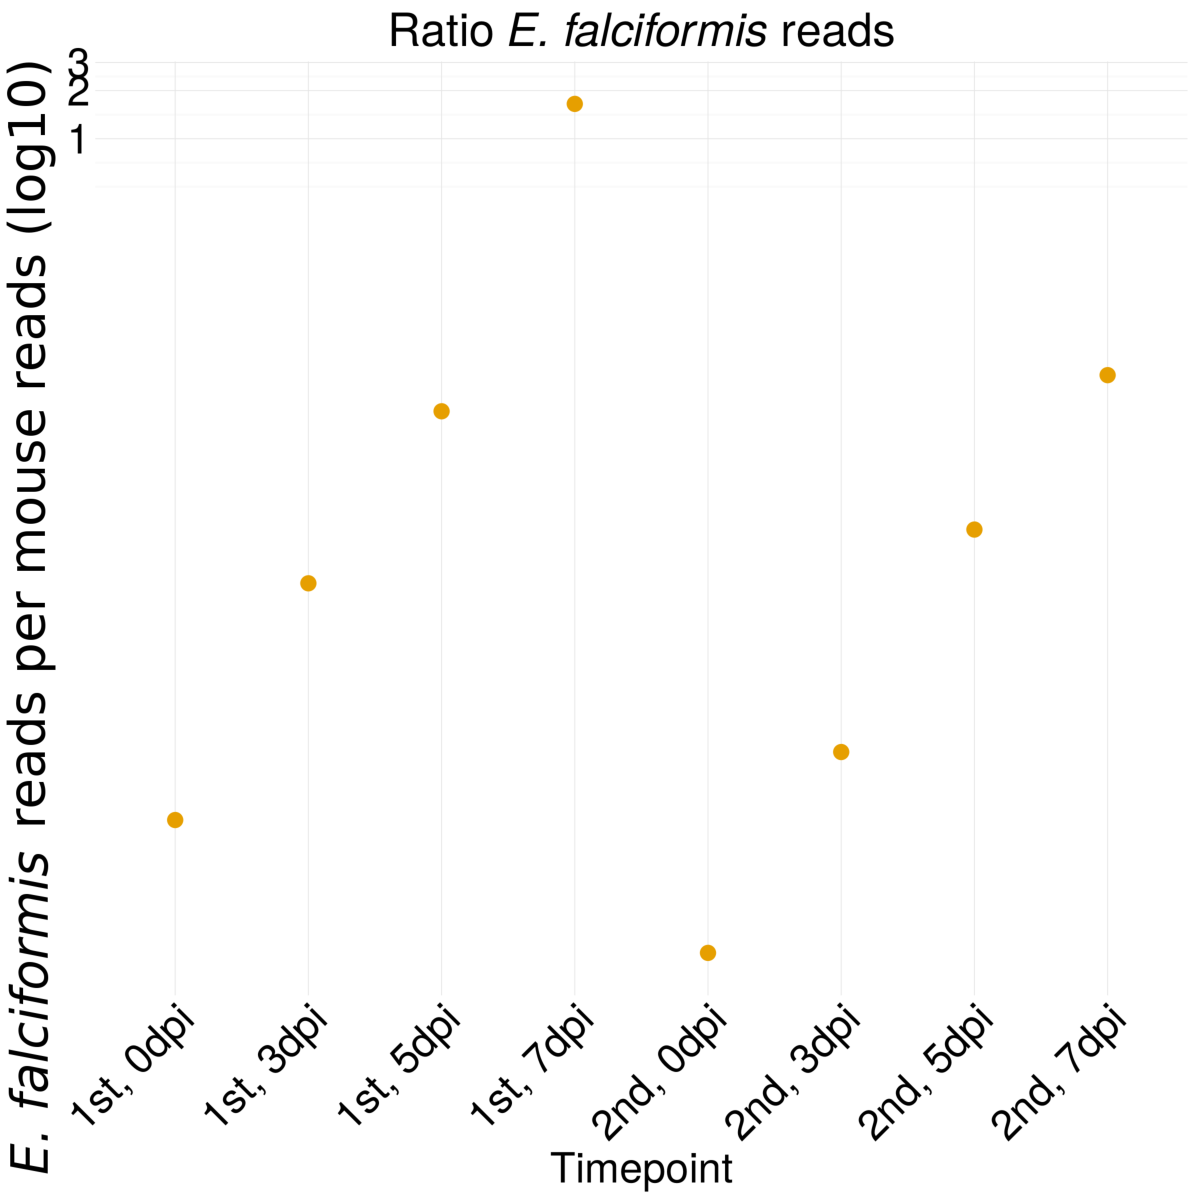
\includegraphics[width=0.5\linewidth]{efmm-ratio}
  \caption{\csentence{Experimental design and outcome of a dual RNAseq experiment}
    read sequences per mouse read sequences for each experimental
    condition. The more advanced the infection is, the higher the
    ratio of parasite reads is, reflecting parasite replication
    between day zero and day seven. ......compare 1st and 2nd
    ....... patterns between Rag and NMRI/C57BL/6?  ........ Values
    are mean of replicates (n=2, if * n=1) on log10 scale. Each sample
    (replicate) consists of mRNA from three different mice.}
  \end{figure}

%%%%%
figure 1 label cotribution of mouse vs. parasite transcripts to the
overall transcriptional output of the analysed tissue for all samples.
%%%%

%% Selecting at most at most 500 genes differentially abundant with
%% lowest FDR (<0.05) are selected. In the next step, the 500 mRNAs from
%% each comparison (or less) are joined. For \textit{E. falciformis} time
%% p.i. comparison, this resulted in 1618 unique genes selected as
%% differently expressed . The 22 genes in the NMRI vs C57BL/6 comparison
%% are not included in the \textit{E. falciformis} life cycle
%% analysis. The same comparisons for mouse yielded 8052 genes in total
%% and 1313 unique ones. In heatmaps, all samples, i.e. also samples
%% which themselves did not have any significantly different mRNAs
%% according to our selection, were included in hierarchical
%% clustering.


%% This might be figure label
%% Scale bar in heatmaps show 0 as mean mRNA abundance for
%% each gene (row). Up (green) and down-regulation (brown) denote number
%% of standard deviations from 0, i.e., row mean. 


\begin{figure}[h!]
%\begin{center}
%\centering
%%	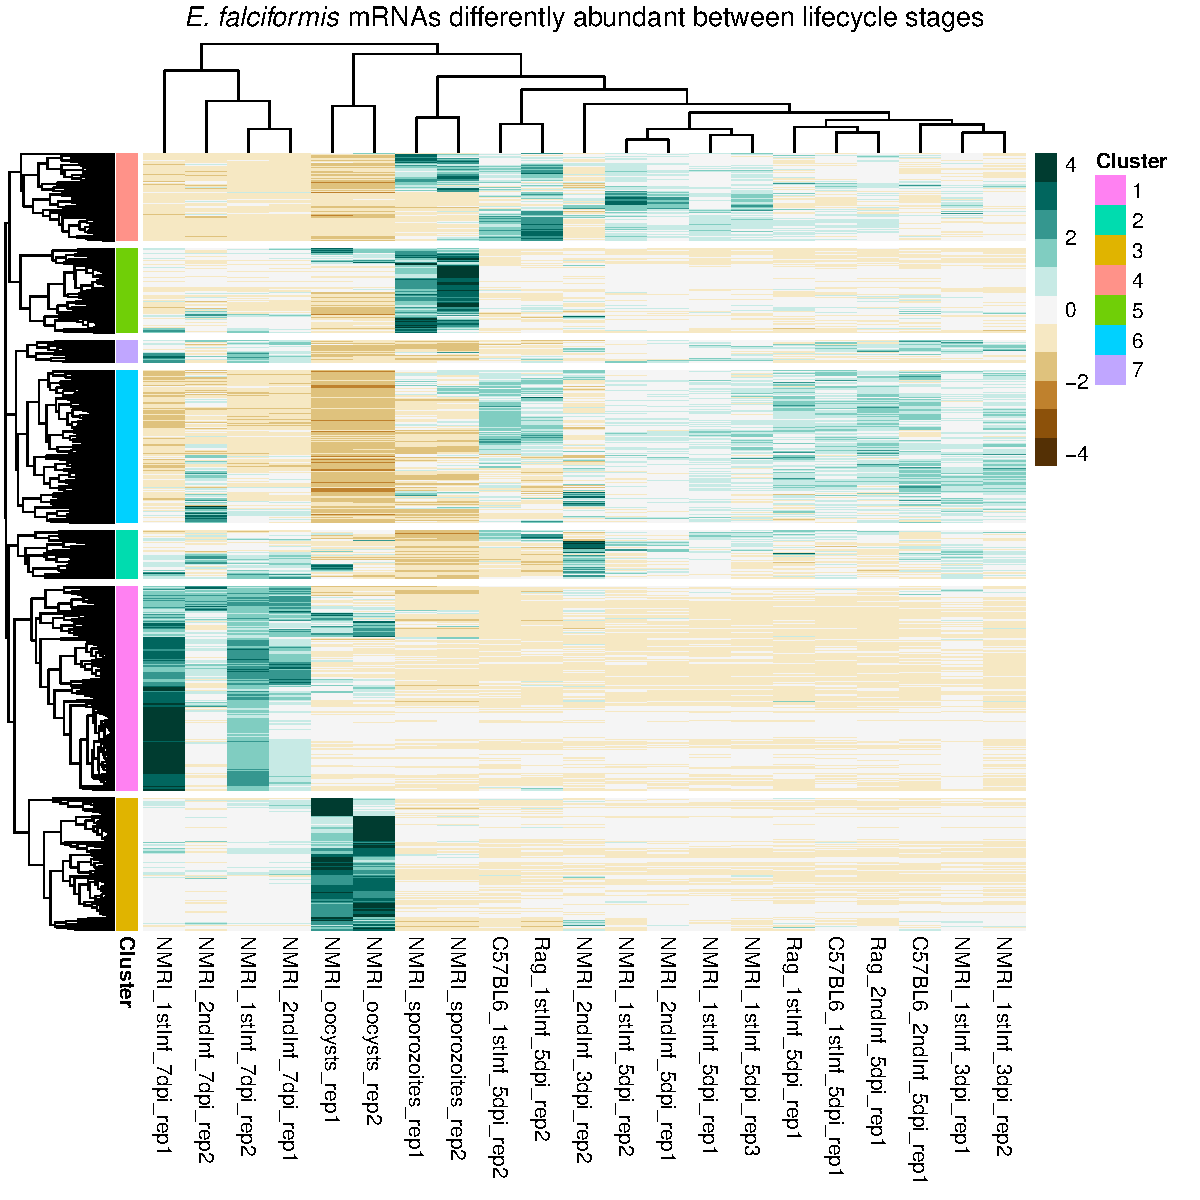
\includegraphics[width=\linewidth]{EfLifecycleHeatmap.pdf}  
	\caption{\textit{E. falciformis} mRNAs with significantly
          different abundance at different times p.i. in NMRI mice
          (see Table 2). Samples cluster according to expected
          developmental state of the parasite, without distinguishing
          between first and challenge infection. Hierarchical
          clustering was set to apply seven gene clusters.}
%\end{center}
\end{figure}


\subsection{Parasite development reflected in mouse data}
\begin{figure}[h!]
%\begin{center}
%\centering
%% 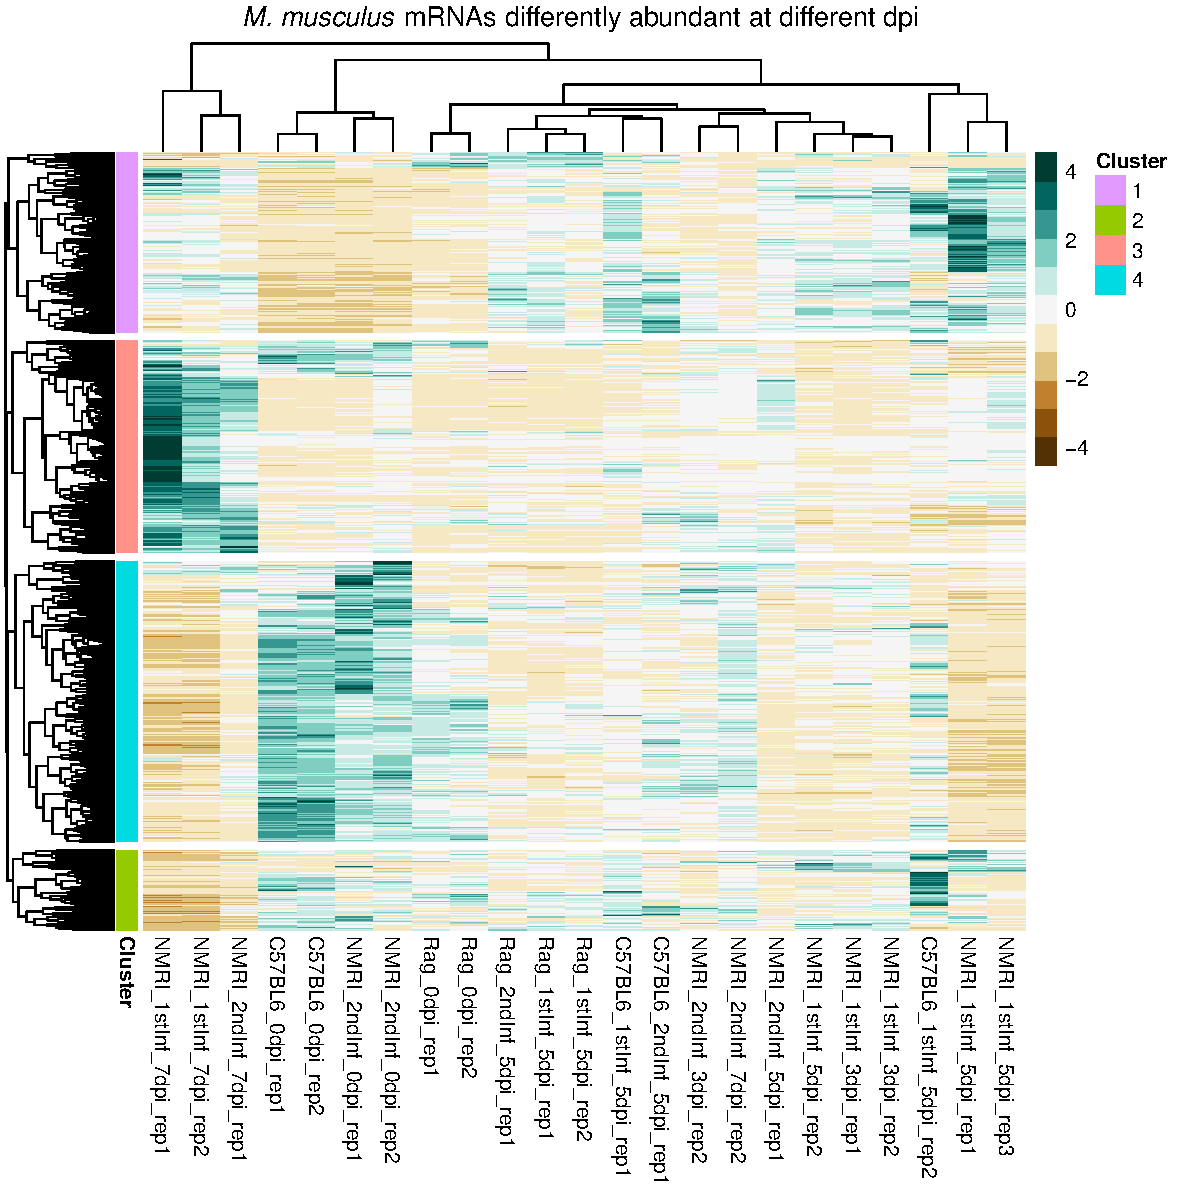
\includegraphics[width=\linewidth]{MmLifecycleHeatmap.pdf}  
\caption{Mouse mRNAs with significantly different abundance at
  different times p.i. in NMRI mice (see Table 2). Samples cluster
  according to expected developmental state of the parasite, without
  distinguishing between first and challenge infection. Rag1-/- mouse
  samples cluster together. Hierarchical clustering was set to apply
  four gene clusters.}
%\end{center}
\end{figure}

When clustering mouse mRNAs which were different in time
p.i. comparisons in Table 2, three out of four samples from day 7
p.i. (NMRI only) cluster together. These samples are characterized by
gene cluster 3 (up) as well as 2 and 4 (down). The fourth day 7-sample
(challenge infection, second replicate) clusters with day 3 and 5
samples. Upon visual inspection of this sample in gene cluster 4, it
diplays a profile similar to non-infected mice. The same sample is
abnormal in the parasite profile (Figure 1). NMRI and C57BL/6
uninfected samples (0dpi) cluster together, defined by gene clusters 4
(up), and 1 (down). Rag1-/- day 0 samples are however less pronounced
in gene cluster 1. Day 3 and 5 samples cluster together, with Rag1-/-
forming a separate group and Rag1-/- non-infected most distant in this
sample cluster.



% \begin{figure}[h!]
 % 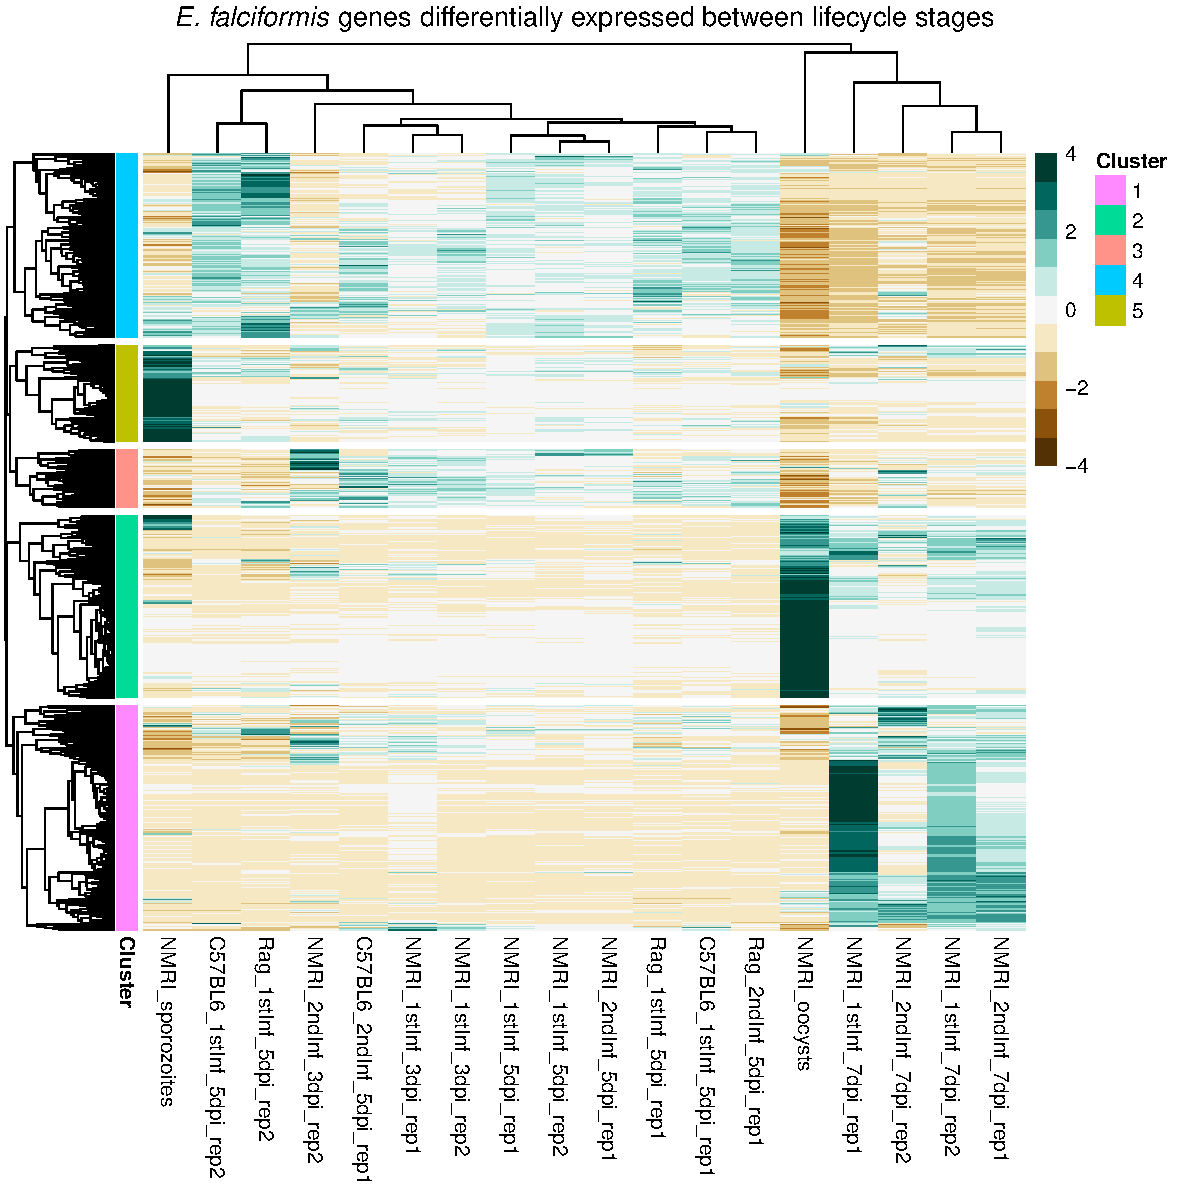
\includegraphics[width=0.7\linewidth]{ef-heatmap} \caption{\csentence{Parasite
 % genes with different mRNA abundance between samples, sorted into
 % five clusters by hierarchical clustering (method = complete,
 % distance = euclidean).}  \textit{E. falciformis} samples from seven
 % days p.i. cluster together (NMRI mice only). These samples have
 % distinct mRNA abundance patterns in all gene clusters, although
 % more pronounced in clusters 1 (up) and 4 (down). Distinct groups of
 % genes also define sporozoites (cluster 5, up) and oocysts (cluster
 % 2, up). mRNA profiles on days three and five p.i. from all three
 % mouse strains cluster together. These samples are distinct from
 % oocysts, NMRI day 7 p.i., and sporozoites, however closest to the
 % latter. On scale bar, 0 is mean mRNA abundance for each gene. Up
 % and downregulation is standard deviations from mean.}  \end{figure}

%\begin{figure}[h!]
%  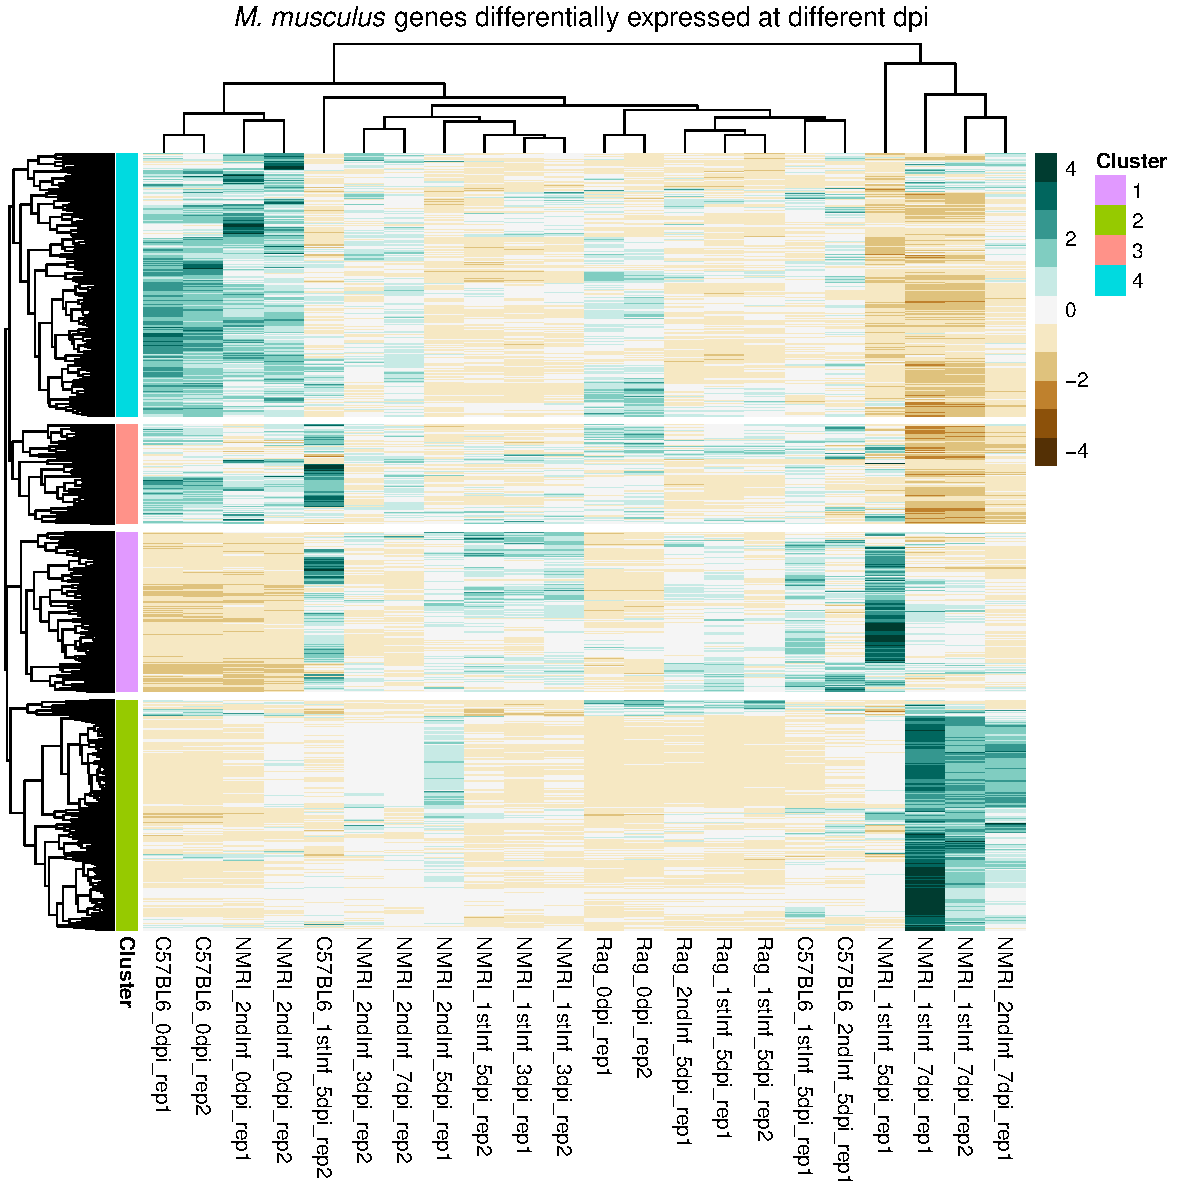
\includegraphics[width=0.7\linewidth]{mm-heatmap} \caption{\csentence{Mouse
%  genes with different mRNA abundance between samples, sorted into
%  four clusters by hierarchical clustering (method = complete,
%  distance = euclidean).}  Three out of four samples from day 7
%  p.i. (NMRI only) cluster together. These samples are characterized
%  by genes in cluster 2 (up), 3, and 4 (down). NMRI and C57BL/6
%  uninfected samples cluster together (left), defined by clusters 3,
%  4 (up), and 1 (down). Rag1-/- samples cluster together. These
%  samples share a weak downregulation of most genes in cluster 2 as
%  well as upregulation of a small group genes in the same
%  cluster. Uninfected Rag1-/- samples are separated from infected
%  ones with distinct profiles in clusters 1, 3, and 4. On scale bar,
%  0 is mean mRNA abundance for each gene. Up and downregulation is
%  standard deviations from mean.}  \end{figure}


%%%%%%%%%%%%%%%%%%%%%%%%%%%%%%%%%%%
%%                               %%
%% Tables                        %%
%%                               %%
%%%%%%%%%%%%%%%%%%%%%%%%%%%%%%%%%%%

%% Use of \listoftables is discouraged.
%%

\newcommand{\bcell}[2][c]{%
  \begin{tabular}[#1]{@{}c@{}}#2\end{tabular}}

\definecolor{LightCyan}{rgb}{0.88,1,1}
\definecolor{LightRed}{rgb}{1,0.88,1}

% Fri Aug 12 11:05:43 2016
\begin{table}[ht]
\centering
\hspace*{-2.5cm}\begin{tabular}{lllllllll}
  \hline
Sample* & \bcell{Sequencing\\method} & batch & \bcell{total\\reads} & \bcell{reads\\mapping\\Mouse} & \bcell{reads\\mapping\\\textit{E. falciformis}} & \bcell{Percentage\\\textit{E. falciformis}}** & \bcell{detected\\ \textit{E. falciformis}\\genes} \\ 
  \hline
NMRI\_2ndInf\_0dpi\_rep1 & GAII & 2 & 108,937,797 & 70,489,674 & 247 & 0.0004 & 1 \\ 
  Rag\_1stInf\_0dpi\_rep1 & hiseq & 3 & 25,362,793 & 18,853,850 & 443 & 0.0023 & 2 \\ 
  C57BL6\_1stInf\_0dpi\_rep1 & hiseq & 3 & 35,731,249 & 25,119,348 & 457 & 0.0018 & 2 \\ 
  C57BL6\_1stInf\_0dpi\_rep2 & hiseq & 3 & 47,085,959 & 34,377,133 & 608 & 0.0018 & 2 \\ 
  Rag\_1stInf\_0dpi\_rep2 & hiseq & 3 & 46,556,156 & 35,233,327 & 676 & 0.0019 & 2 \\ 
  NMRI\_2ndInf\_0dpi\_rep2 & hiseq & 3 & 58,122,244 & 40,794,245 & 3,406 & 0.0083 & 51 \\ 
  \rowcolor{LightCyan}
  NMRI\_2ndInf\_3dpi\_rep1 & hiseq & 3 & 57,934,016 & 40,544,287 & 4,803 & 0.0118 & 95 \\ 
  \rowcolor{LightCyan}
  NMRI\_2ndInf\_5dpi\_rep2 & hiseq & 3 & 63,965,539 & 48,289,181 & 10,941 & 0.0227 & 407 \\ 
  \rowcolor{LightRed}
  NMRI\_1stInf\_0dpi\_rep1 & GAII & 1 & 82,364,585 & 55,176,243 & 17,954 & 0.0325 & 701 \\ 
  NMRI\_2ndInf\_3dpi\_rep2 & hiseq & 3 & 65,548,826 & 46,171,909 & 29,548 & 0.0640 & 1,580 \\ 
  NMRI\_2ndInf\_7dpi\_rep2 & hiseq & 3 & 67,487,466 & 51,722,265 & 40,091 & 0.0775 & 1,836 \\ 
  Rag\_1stInf\_5dpi\_rep1 & hiseq & 3 & 38,651,359 & 29,982,453 & 63,024 & 0.2098 & 2,548 \\ 
  Rag\_1stInf\_5dpi\_rep2 & hiseq & 3 & 34,779,832 & 25,297,803 & 99,000 & 0.3898 & 2,828 \\ 
  C57BL6\_1stInf\_5dpi\_rep1 & hiseq & 3 & 40,904,388 & 29,319,604 & 185,969 & 0.6303 & 4,173 \\ 
  Rag\_2ndInf\_5dpi\_rep1 & hiseq & 3 & 50,049,848 & 37,093,621 & 192,856 & 0.5172 & 4,167 \\ 
  C57BL6\_1stInf\_5dpi\_rep2 & hiseq & 3 & 29,511,368 & 18,062,349 & 215,696 & 1.1801 & 3,823 \\ 
  C57BL6\_2ndInf\_5dpi\_rep1 & hiseq & 3 & 35,148,432 & 25,660,184 & 262,909 & 1.0142 & 4,563 \\ 
  NMRI\_1stInf\_3dpi\_rep1 & GAII & 1 & 73,236,430 & 49,993,358 & 394,384 & 0.7827 & 5,220 \\ 
  NMRI\_1stInf\_3dpi\_rep2 & GAII & 2 & 160,709,694 & 117,791,044 & 413,051 & 0.3494 & 4,862 \\ 
  NMRI\_1stInf\_5dpi\_rep2 & GAII & 2 & 119,902,722 & 76,419,774 & 794,570 & 1.0290 & 5,333 \\ 
  NMRI\_2ndInf\_5dpi\_rep1 & GAII & 2 & 230,773,955 & 143,186,486 & 1,846,840 & 1.2734 & 5,533 \\ 
  NMRI\_2ndInf\_7dpi\_rep1 & hiseq & 3 & 70,366,762 & 41,467,146 & 8,634,201 & 17.2335 & 5,875 \\ 
  NMRI\_1stInf\_5dpi\_rep1 & GAII & 2 & 76,702,168 & 47,037,087 & 8,669,701 & 15.5631 & 5,700 \\ 
  NMRI\_sporozoites\_rep2 & GAII & 0 & 19,551,681 & 8,656 & 11,470,604 & 99.9246 & 5,513 \\ 
  NMRI\_1stInf\_5dpi\_rep3 & GAII & 0 & 191,099,180 & 83,735,624 & 27,839,458 & 24.9513 & 5,784 \\ 
  NMRI\_1stInf\_7dpi\_rep1 & GAII & 1 & 66,505,514 & 3,310,666 & 39,400,884 & 92.2488 & 5,932 \\ 
  NMRI\_sporozoites\_rep1 & GAII & 1 & 67,325,397 & 4,334 & 43,774,401 & 99.9901 & 5,825 \\ 
  NMRI\_oocysts\_rep1 & GAII & 1 & 68,859,802 & 3,805 & 49,653,065 & 99.9923 & 5,695 \\ 
  NMRI\_oocysts\_rep2 & GAII & 0 & 151,090,783 & 18,524 & 71,019,860 & 99.9739 & 5,777 \\ 
  NMRI\_1stInf\_7dpi\_rep2 & GAII & 1 & 139,749,046 & 21,699,324 & 73,539,445 & 77.2159 & 5,943 \\ 
   \hline
\end{tabular}
\begin{tablenotes}[flushleft]\footnotesize\singlespacing
\item{*} sample names are given as a) mouse strain b) first or challenge
  infection c) days post infection (dpi) and d) replicate number
  seperated by undersocre . \\
\item{**} percentag mapping \textit{E. falciformis} is given as percentage in total mapping reads
\end{tablenotes}
\end{table}
\hspace*{+2.5cm}





%%%%%%%%%%%%%%%%%%%%%%%%%%%%%%%%%%%%%%%%%%%%%%%%%%%%%%%%%%%%%%%%%%%%%%%%%%
%% 	NUMBER OF GENES DIFFERENT IN DIFFERENT COMPARISONS	
%%%%%%%%%%%%%%%%%%%%%%%%%%%%%%%%%%%%%%%%%%%%%%%%%%%%%%%%%%%%%%%%%%%%%%%%%%
%% I like this table. Looks good and transprorts the right kind of
%% information

\clearpage
\section{mRNA abundance differences between different experimental groups}
\setlength{\tabcolsep}{8pt}
\begin{table}[H]
\small
\begin{center}
\caption{mRNA abundance differences between different experimental groups.}
%\label{tab:table3}
\begin{tabular}{*3l}    \toprule
\textit{Day post infection} & \textit{Ef} genes different & Mouse genes different \\ 
	\textit{comparisons} 	    & (FDR$\leq$1\%) &  (FDR$\leq$1\%/5\%) \\ \midrule
	NMRI 0 vs NMRI 3		& NA   & 274 \\
	NMRI 0 vs NMRI 5		& NA   & 1736 \\
	NMRI 0 vs NMRI 7		& NA   & 2802 \\
	NMRI 3 vs NMRI 5     		& 111  & 1 \\
	NMRI 3 vs NMRI 7  		& 1385 & 1407 \\ 
	NMRI 5 vs NMRI 7  		& 1895 & 873 \\ 
	C57BL/6 0 vs C57BL/6 5		& NA	& 914 \\
	Rag1-/- 0 vs Rag1-/- 5		& NA	& 45 \\ \midrule
\textit{Day post infection,} & 		 & 		 \\ 
\textit{parasite relevant comparisons} 	    & 		&  \\ \midrule
	Oocysts vs NMRI 3  	& 3310 & NA \\  
	Oocysts vs NMRI 5	& 3605 & NA \\ 
	Oocysts vs NMRI 7	& 3085 & NA \\ 
	Oocysts vs sporozoites  & 3421 & NA \\
	Sporozoites vs NMRI 3 	& 1663 & NA \\
	Sporozoites vs NMRI 5 	& 1605 & NA \\
	Sporozoites vs NMRI 7 	& 2473 & NA \\ \midrule
\textit{First and second infection} & 		 & 	 \\ 
\textit{comparisons} 	    & 		& 	\\ \midrule
	NMRI 3 1st vs NMRI 3 2nd  	& 0  & 5 \\
	NMRI 5 1st vs NMRI 5 2nd  	& 0  & 1 \\
	NMRI 7 1st vs NMRI 7 2nd  	& 0  & 902 \\
	C57BL/6 1st vs C57BL/6 2nd (day 5) & 0 &  mouse \\
	Rag1-/- 1st vs Rag1-/- 2nd (day 5) & 0 & mouse  \\ \midrule
\bottomrule
	\hline
\end{tabular}
\end{center}
\end{table}




%%%%%%%%%%%%%%%%%%%%%%%%%%%%%%%%%%%
%%                               %%
%% Additional Files              %%
%%                               %%
%%%%%%%%%%%%%%%%%%%%%%%%%%%%%%%%%%%

\section*{Additional Files}
  \subsection*{Additional file 1 --- Raw and normalized counts }
  Raw counts of reads mappins to the \textit{E. falciformis} and mouse
  genome for individual samples in our study. Normalized counts for
  seperately for the host and parasite mappings (three compressed csv
  files).
  
  \subsection*{Additional file 2 --- Results of statistical tests (edgeR) }
  Focal contrast, fold-changes, likelihood ratio in/excluding this
  difference in models, p-values , and false discovery rates (adjusted
  p-values) are given for all tested contrasts (one compressed csv
  file).
  
  \subsection*{Additional file 3 --- Additional methods and resuts }
  % this would be cool but requires special referencing in the text
  % (hard to keep track and hard to fit in the journals referencing
  % system). But we can try.
  Document containing additonal figures and summary tables (pdf).

\subsection*{Additional file 4 --- Results of enrichment analyses (topGO)}
  Tables listing all tested gene sets and resulting significatn GO
  terms.
  
  
\end{backmatter}
\end{document}
